\documentclass[a4paper,11pt, oneside]{article}   % list options between brackets
\usepackage{fullpage}
\usepackage[utf8]{inputenc}

\usepackage{graphicx}
% type user-defined commands here
\usepackage{indentfirst}

\usepackage{multirow}

\usepackage{url}
\usepackage{float}

\usepackage[colorlinks]{hyperref}
\hypersetup{
   citecolor={black},
   linkcolor={black},
   urlcolor={black},
   pdfpagemode={UseOutlines}
}

%% Handle links to references better.
\usepackage[all]{hypcap}

\usepackage{index}

\usepackage{subfigure}

\usepackage{caption}
\captionsetup{width=0.9\textwidth}

\newcommand{\f}[1]{\mbox{\texttt{#1}}}
\newcommand{\ttf}[1]{\texttt{#1}}
\newcommand{\HRule}{\rule{\linewidth}{0.5mm}}

\begin{document}

\begin{titlepage}

\begin{center}


% Upper part of the page

\includegraphics[width=0.50\textwidth]{./figures/logo}\\[3 cm]

\textsc{\large Big Data}\\[1.5cm]

{\Large Project Report}\\[0.5cm]


% Title
\HRule \\[0.4cm]
{ \huge \bfseries Weather Dashboard}\\[0.2cm]

\HRule \\[1.5cm]

% Author and supervisor
\begin{minipage}{0.5\textwidth}
\begin{flushleft} \large
\emph{Authors:}\\
Aubry \textsc{Cholleton}\\
Jonathan \textsc{Duss}\\
Anders \textsc{Hennum}\\
Alexis \textsc{Kessel}\\
Quentin \textsc{Mazars-Simon}\\
Cédric \textsc{Rolland}\\
Orianne \textsc{Rollier}\\
David \textsc{Sandoz}\\
Amato \textsc{Van Geyt}
\end{flushleft}
\end{minipage}
\begin{minipage}{0.4\textwidth}
\begin{flushright} \large
\emph{Professor:} \\
Christoph \textsc{Koch} \\
\vspace{1cm}
\emph{Supervisor:} \\
Amir \textsc{Shaikhha} \\
\end{flushright}
\end{minipage}

\vfill

% Bottom of the page
{\large May 20, 2014}

\end{center}

\end{titlepage} 

\tableofcontents
\newpage


%\input{./introduction.tex}

\section{Data Retrieval}
\subsection{Looking for data}
Initially, the project idea was to get Alps weather information from social networks using natural language processing. Hence we first looked how to mine Twitter, Facebook, Instagram or Camptocamp. We also searched for other datasources such as the \emph{Institute for Snow and Avalanche Research} (SLF), MeteoSuisse or ski resorts. After discussion and clarification with our TA, the scope and goal of our project changed in order to get closer to a \emph{Big Data} project. Hence we needed to process a big dataset and the \emph{Integrated Surface Database} from NOAA seems to be the one.

\subsection{The \emph{Integrated Surface Database}}
The \emph{National Oceanic and Atmospheric Administration} (NOAA) is the US agency responsible for the weather surveillance and forecast. They have a \emph{National Climatic Data Center} (NCDC), “responsible for preserving, monitoring, assessing, and providing public access to the Nation's treasure of climate and historical weather data and information”. One of their dataset is the \emph{Integrated Surface Database} which has data not only for the USA territories, but for the whole world (20,000 stations). We can access this dataset under the following condition, which we fulfill.
\begin{quote}
“The following data and products may have conditions placed on their international commercial use. They can be used within the U.S. or \textbf{for non-commercial international activities without restriction}. The non-U.S. data cannot be redistributed for commercial purposes. Re-distribution of these data by others must provide this same notification.”
\end{quote}
The data is accessible by FTP at \url{ftp://ftp.ncdc.noaa.gov/pub/data/noaa/} using anonymous login. There is one directory per year and within each directory one file per weather station. Within a file, one line correspond to one data record of the station at a specific time.

All stations are listed in the file \texttt{ish-history.txt} with, among other attributes, their coordinates and the country in which they are located.

Every station can have two IDs: the \emph{Air Force Datsav3 station number} (USAF) (6 figures) or the \emph{NCDC WBAN number} (WBAN) (5 figures). Most stations have only one of these two IDs (the other being set to 9s). Hence we defined the ID of a station as being the combination of the two IDs, which guarantee uniqueness.

It is important to note that despite the fact that each stations has precise coordinates, each line entry in the dataset give the coordinates again because a station might be slightly moved.

\subsection{Downloading the data}
The dataset is over 500GB large when uncompressed. As we only have 300GB on our server, we couldn't download the whole dataset. In order to have a sample dataset, we downloaded 10 years (2004-2013) of data for Switzerland, which is around 2GB large. Then we downloaded 39 years (1975-2013) of data for the USA, which is around 200GB large. We can notice that these 39 years of data for the USA are a big part of the whole dataset. We can therefore deduce that they richer (more frequent sampling).

\begin{figure}[htb]
	\centering
	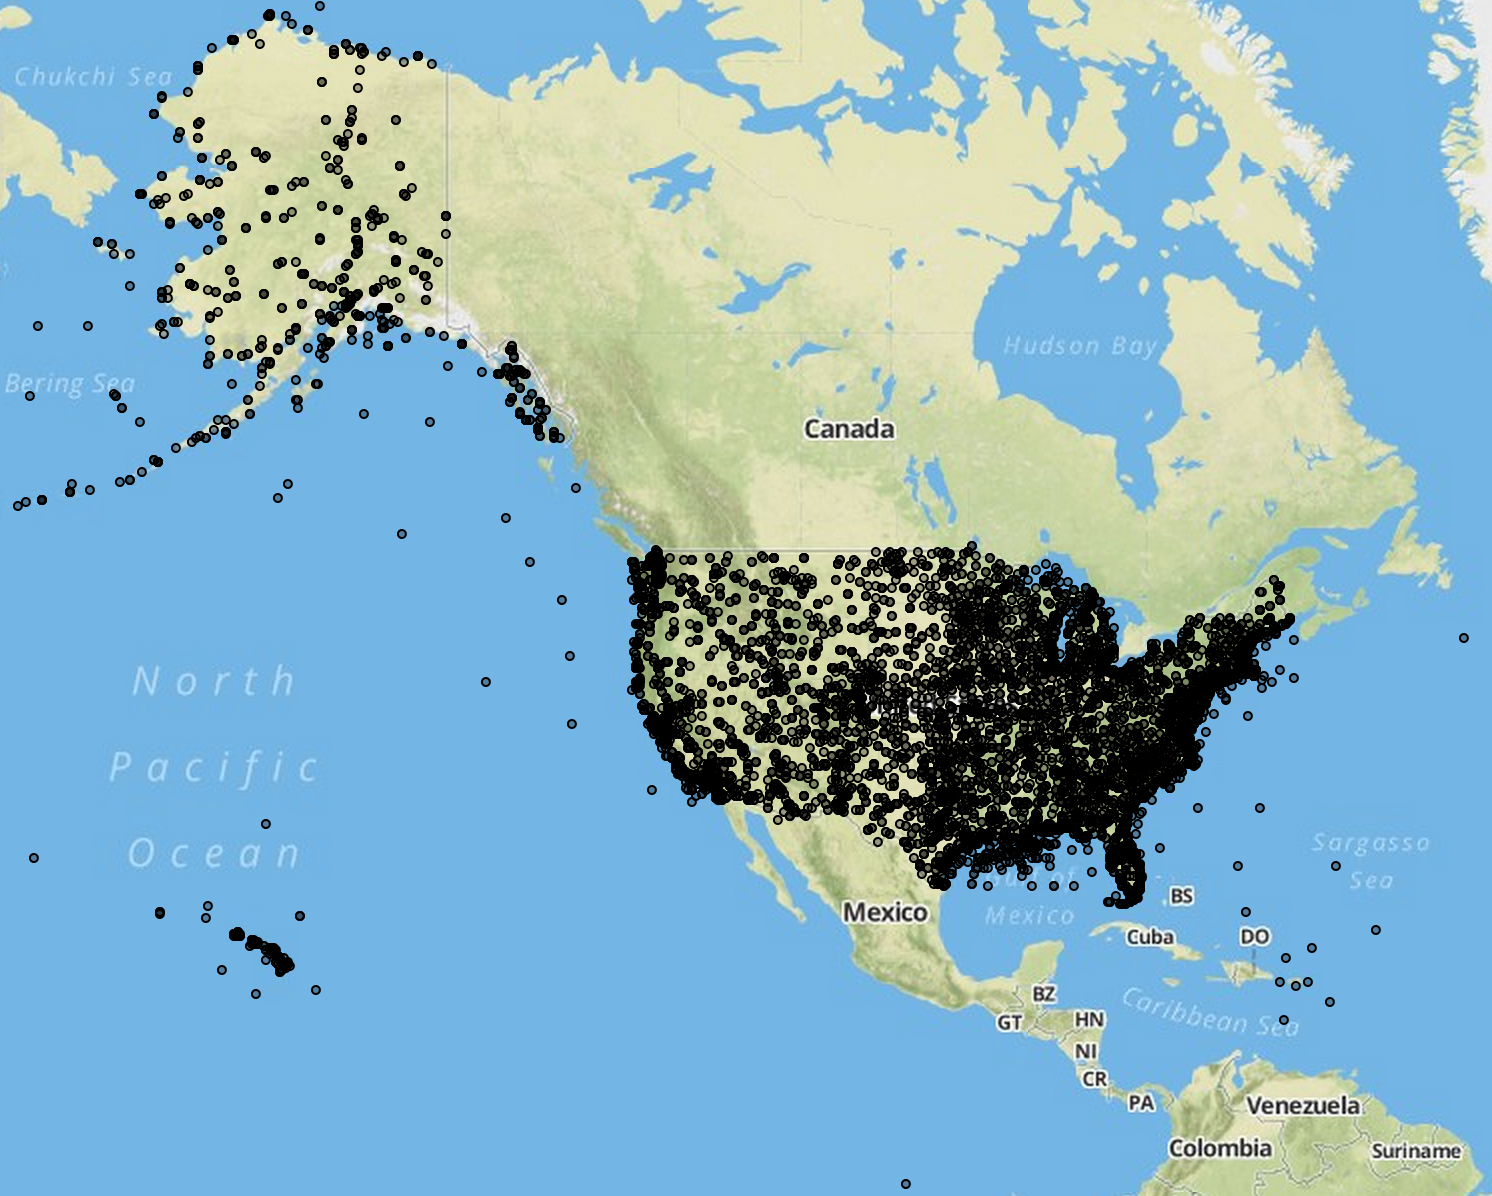
\includegraphics[width=0.9\textwidth]{figures/USStations.png}
	\caption{Stations categorized as being in the USA}
\end{figure}

To proceed the download from the NOAA FTP server to our server, we wrote a Shell script taking in argument the \texttt{filename} of a file containing a list of the stations we want and the \texttt{year} for which we want the data. As all the stations are not active, there will not necessary be a file for each station in our list. Hence, before downloading, the script compute the intersection between the stations in our list and the files available on the FTP server. This will improve the downloading as it will not ask for files which doesn't exist.
%\documentclass[12pt]{article}

%\usepackage{hyperref}
%\usepackage{graphicx}
%\usepackage{float}

%\begin{document}
\section{Wikipedia}
In this section, we will describe each step of the procedure from the Wikipedia data dump to displaying the information on the website.
\begin{figure}[H]
    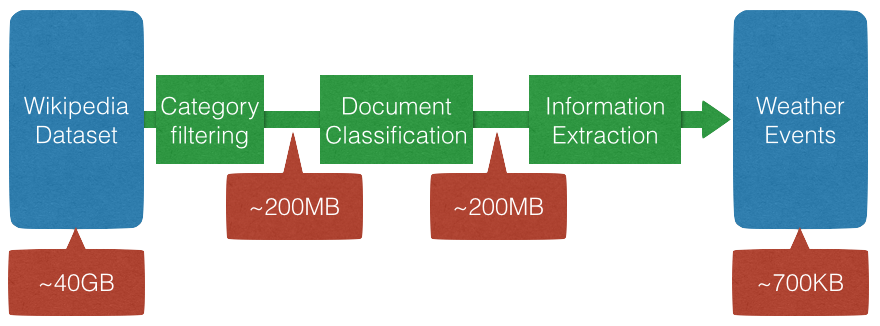
\includegraphics[width=\textwidth]{figures/wiki-flow.png}
    \caption{Overview of Wikipedia information extraction}
     \label{fig:wikiflow}
\end{figure}
\subsection{Available data}
It is possible to download a dump of all English Wikipedia articles, without edit history, from \href{https://meta.wikimedia.org/wiki/Data_dump_torrents#enwiki}{this webpage}. We used the dump from February 3rd, 2014, the latest available when we started the project. It consists of a single XML file which is 10GB compressed, 40GB uncompressed. 
\subsection{Filtering articles}
Obviously, most of Wikipedia articles are irrelevant to our task of find information on weather events, that is why we must first filter the dataset. 
\subsubsection{Filtering based on articles' categories}
The easiest way to prune off topic articles, it to look at their category. Unfortunately, categories on Wikipedia are not hierarchically well organized, so we cannot start from a top category such as ``weather event'' and get a list of every relevant subcategories. Indeed, categories may loop or diverge to another subject.\\\\
Knowing this, we decided to filter categories based on a defined set keywords: "blizzard", "cyclone", "hurricane", "typhoon", "derecho", "drought", "nor'easter", "storm", "tornado", "heat wave", "cold wave", "weather event". \\\\
An article belonging to a category which contains one of those keyword is jugged relevant. This allows us to filter out most irrelevant articles, even if there are some false positives (e.g. football players affiliated to a team called ``The Hurricanes'').\\\\
Implementation wise, this filtering consist of a single MapReduce job where the mapper only emits an article if it is relevant, and the reducer combines the articles it receives into a single XML file for each keyword. 
After running the job (usually takes less than 5 minutes), we now only have around 200MB of data, which allows us to do document classification in reasonable time, and filter out the remaining off-topic articles.\\ 
We use Mahout's XMLInputFormat which provides an easy way to split the input into multiple articles delimited by the \texttt{<article>} and \texttt{</article>} tags and send them to the mapper.
\subsubsection{Filtering using document classification}
ORIANNE
\subsection{Extracting information}
Now that we have only relevant articles, we can start extracting information. \\
The general idea is to first locate the article's infobox which, if it exists, usually provides detailed information on date and location of the event (date formed, date dissipated, areas). If there is no infobox, or we still need more information, we try to extract it from the article's title, and finally, as a last resort we try to find the information in article's body.\\\\
We only use a mapper to extract information, the reducer is only used to combine the results.
After extraction, we have a single CSV file (separated by tabs) containing the following columns: title, category, start date, end date, location. At this point we have less than a megabyte of data. Running this job usually takes less than two minutes.
\subsubsection{Extracting dates}
To extract dates we use multiple regexes, to cover the range of available date formats (DD/MM/YYYY; YYYY$|$MM$|$DD; m dd, YYYY; dd m YYYY; etc.). We then convert them all to a predefined date format: DD/MM/YYYY. 
\subsubsection{Extracting locations}
To extract location, we use a regex based on the lists of continents, countries and american states as well as their corresponding demonyms given in \href{http://en.wikipedia.org/wiki/List_of_adjectival_forms_of_place_names}{this Wikipedia article}.
\subsection{Displaying information}
In order to display correctly the information, we first run a small python that creates http link for each article's title (\texttt{<a href='http://en.wikipedia.org/wiki/\$TITLE'> \$TITLE </a>}), and get the number of references of an articles from Wikipedia using a GET request (\texttt{https://en.wikipedia.org/wiki/Special:WhatLinksHere/\$TITLE}).\\
We then sort the articles by their number of reference, to display most important events first\\\\
On the webpage, we display the information as an HTML table whose rows can be easily filtered to show only relevant events.
\subsection{Results}
The quality of the result greatly depends on the article's category. For example, each hurricane usually has its own article which almost always contains an infobox with precise start/end date as well as areas affected, whereas tornadoes are usually grouped under the same article where extracting information is harder (e.g. tornadoes of  2012); also for some weather events (such as cold/heat waves) it is hard to define clear start/end dates.
%\end{document}

\section{Rainfall}
This part of the project was taken care of by Amato Van Geyt. The goal of this was identifying different anomalies in the rainfall in the USA in a given time period. The time period we choose was 1970 until 2013 as the used datasets seemed to have the most available and reliable data in this period. \\ \\
The used dataset was initially the original noaa-dataset (\url{ftp://ftp.ncdc.noaa.gov/pub/data/noaa/}) but many problems were encountered with this dataset, especially for the rainfall. First of all was all the data organised by year which made it hard to debug as for finding anomalies we need to be able to quickly compare a certain value with values at the same place but at different times, something this dataset hindered us in. The records themselves were also very chaotically organised and contained much useless information giving cause to long and error-prone processing. The worst of all though was the fact that the rainfall wasn't given per day but for a certain time-period expressed in hours. As this time-period varied a lot among the different weather-stations or even for the same time-period and as there were gaps of data this gave cause to very erratic results. This gave cause to choosing for a new dataset which was aggregated on the previous one. \\ 
The new dataset (\url{ftp://ftp.ncdc.noaa.gov/pub/data/ghcn/daily/}) contained essentially the same data but sorted by weather-station (one file per station) and each line of that file told us exactly the daily values for a certain weather measure for a given month of a given year. This allowed for very easy parsing and processing. The files were much smaller as well and easier for debugging. The final results are based on this data and can be seen on the site.\\ 

The way how the results are obtained is simple. By using two phases of MapReduce we identify for every station the average and standard deviation of all the values over all the years in the data. This can be done for the value per day, or the value per month, which is the average of all daily values. As there was still some 'dirty' or missing data we did some filtering on the quality before using it in our computation. And if saw that the amount of data used to calculate the standard deviation and average was too small, we dropped it as it was too error-prone. Then we used a parameter, entered via the command line to determine what we would see as an anomaly and what not. This value would be the amount of standard deviations the value had to be away from the average to be seen as an anomaly. After some experimenting we saw that the best value for our daily anomalies was 6 and for our monthly anomalies 3. Our final output was a text file per weather station which contained all the anomalies we found for it, one per record. The record contained the time, the station-ID, the value, the standard deviation and its normal average value. \\
As this did not contain the coordinates of the station and the name of the station yet we had to make an additional MapReduce-phase which took our previous output as input and added this additional data to every record while also re-organising it. The last step we had to do after this was to do another processing step in order to visualize it on a map. In order to do this, in an uniform way with the other parts of the project, we use GeoJSON. After this was done, the only thing remained was plugging it into the already existing map, doing some small modifications. The final result can be seen in Figure \ref{fig:rainfall1}. The anomaly found in it was indeed an anomaly as the hurricane Emily made a passage through North Carolina during those days, as shown in the Wikipedia-report in Figure \ref{fig:rainfall2}.
\begin{figure}[ht]
\centering
\makebox[\textwidth][c]{
  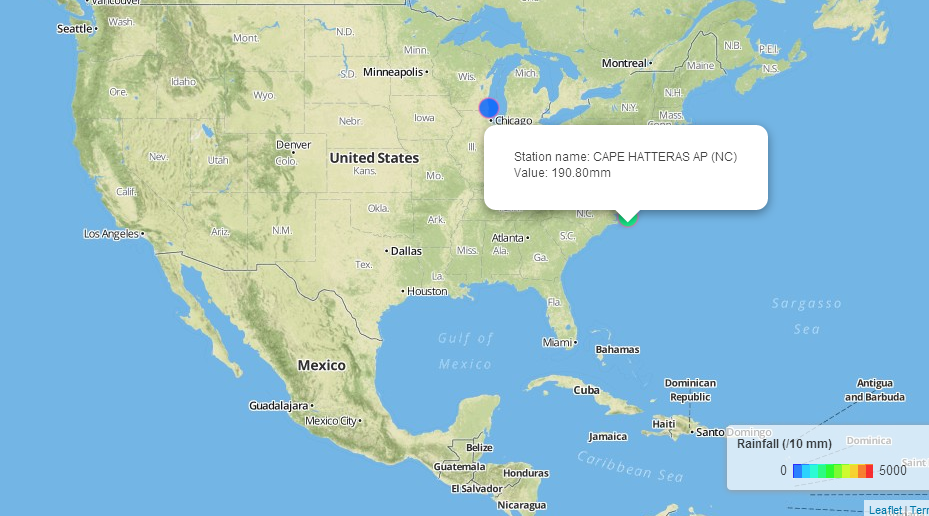
\includegraphics[width=17cm]{figures/rainfall1.png}
}
\caption{The rainfall anomalies on 31/08/1993}
\label{fig:rainfall1}
\end{figure}
\begin{figure}[ht]
\centering
\makebox[\textwidth][c]{
  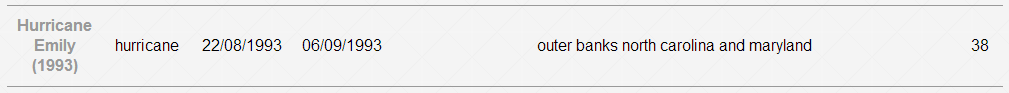
\includegraphics[width=17cm]{figures/rainfall2.png}
}
\caption{The wikipedia-report of hurricane Emily}
\label{fig:rainfall2}
\end{figure}

\documentclass{article}

\usepackage{enumerate}
\usepackage{amsmath} 
\usepackage[utf8x]{inputenc}

\usepackage{graphicx}
\setlength{\parindent}{0 pt}
\usepackage[usenames,dvipsnames]{color}
\usepackage{color}


\begin{document}

\section*{Snow accumulation}

\subsection*{Ideas constraint by available data}
The first idea was to collect extreme snow depth events (snow on the floor) in the US, but a problem appeared pretty soon. Not all weather stations measure it. The first MapReduce Job simply computes how many records there are about snow. It appears that there are only around 10000 records per year in the last decades. But with the age, the number decrease and end to be too small. To find a trend, it was needed to have enough stations from the beginning which was not the case.  \\

To bypass the problem, the idea was to estimate snowfalls from precipitations. When it snows, it is melted and this gives what is called the water-equivalent. To check if there are enough precipitation data, a similar map/reduce has been written to count the records. The NOAA provides a table to convert approximately a water height into a snow equivalent based on the temperature.

\subsection*{ Data Analysis}
The first map/reduce job takes in input raw data and output the daily snow accumulation. Some records can be erroneous, missing in which case the data are excluded. To have more precise results, the snow cumulation is computed from the difference of snow depth if it is provided. In the other case, the snowfall is estimated from the precipitation data and the temperature.

To show something interesting on a map, the daily representation does not fit. This is why 2 more jobs have been written to compute the weekly and monthly snow accumulation. It shows how much it snowed during a given week or month and it is possible to see the snowstorms, and also how intensive and extensive they were.\\


Finally we wanted to show a snow trend over 35 years for the whole country. Two approaches were tested. The first one computes the average snow accumulation for each month of each year. The average was computed over all stations. But there is a problem, snow stations were added and if more station are added in a snowy area, it would produce biased results. The second only takes in account stations where there are snow, when the measure was made. Again it produces biased results. If a whole region does not have snow during a year, or on the contrary, if it snows over a wide area  where snow is usually rare, the result won't take it into account. To obtain correct results, it would have been necessary to take a set of station existing from 1980 to today. Unfortunately, the time was missing to fix it this way. 




%The first mapper take in input a file containing all data about one station. It checks if there is snow depth data in which case, it compute the difference with the last known value if it is not too old. In case there is no measure about the snow depth or if the last measure is too old, it checks if there is any precipitation data and compute the snow equivalent using the temperature. The mapper outputs the result and the key
%The reducer receive a list of snowfalls for a given day for a given station. It add all the measure and output it. The output corresponds to how much it snowed a given day at a given station.




\end{document}

\section{Nearest Neighbors}

\subsection{Why?} % (fold) \label{sub:why_}

% subsection why_ (end)
The main purpose of implementing nearest neighbor, is to find similar weather
periods in the history and possibly find patterns in the climate. This is useful
in terms of understanding the climate and to forecast specific events. 

As an example, here in Switzerland, it could be useful in terms of avalanche
danger. If most of the nearest neighbors of the current winter so far, led to
many and massive avalanches, it is reason to believe that also the current
winter can become a such a winter. By knowing this, it would be possible to take
action before the events occur. The same method can be used to forecast events
like floods or drought.  

It can also be used to find patterns in the climate such as cycles and periodic
structures. 

TODO: Rewrite to better language

\subsection{Implementation} % (fold) \label{sub:implementation}

The k-nearest neighbor is a fairly simple algorithm. You choose a metric,
calculate the distance from the reference node to all the other's, and pick the
$k$ nearest neighbors. This has been done more or less straight forward.

In this case a node is a period of time. We fixed the period to one month, such
that you can pick one month for a specific year, and then find the most similar
months for the other years. Often climate data is summarized by month, so this
makes it easy to find data to compare with.

Next question is to determine how many intervals the period of time should be
divided into. Should we compare averages for an hour, a day, a week, or just one
value for the whole month? For a small region (a few stations) and a short
period of time (a day), then comparing hour by hour could make sense and give
good results. But for a large region (thousands of stations) and for a longer
period (a month), this will mostly just return noise. Here, the method is
implemented with a period option so one can choose how many periods a month
should be divided into. The final results is run with this set to 1, meaning
that averages for the whole month is used. 

TODO: add figure shows how this was implemented with map reduce on Hadoop. Write
some more and clean language.
% subsection implementation (end)

\subsection{Results} % (fold) \label{sub:results}

TODO: Present some results with some figures to show that it works.

% subsection results (end)

\section{User interface}
The user interface is divided in two parts: the map and the graph. The map is a visualization of the following computations: temperature anomalies, snow cumulation, rainfall and storms. The graph is a visualization of the nearest neighbors.

\subsection{Map engine}
At first we tried to include maps using OpenLayers 3, which is quite promising but still in beta. We faced some problems due to different projections system which gave us some hard time. Hence we finally switched to Leaflet + Mapbox which works pretty well.

\subsection{}

\section{Tasks distribution}
\begin{tabular}{|l|p{10.5cm}|}
\hline
\textbf{Student} & \textbf{Tasks s-he accomplished} \\
\hline
Aubry Cholleton & \begin{itemize}
	\item Find NOAA datasets on the web and resources about it.
	\item Write a generic algorithm to filter and aggregate data from NOAA (temporally and spatialy), perform some statistics and classification of extreme events and output the results.
	\item Apply this algorithm to temperature anomalies.
	\item Write python scripts to convert Hadoop output to geoJSON, to transform coordinate systems and to interpolate data.
	\item Visualizations of temperature anomalies in javascript using leaflet for the map and geoJSON file format.
\end{itemize}\\
\hline
Jonathan Duss & \\
\hline
Anders Hennum & \\
\hline
Alexis Kessel & \\
\hline
Quentin Mazars-Simon & \begin{itemize}
	\item Data retrieval from Wikipedia and upload to our servers
	\item Wikipedia articles filtering based on categories
	\item Wikipedia information extraction
	\item Wikipedia visualisation (Python + Javascript)
\end{itemize}\\
\hline
Cédric Rolland &  \\
\hline
Orianne Rollier & \\
\hline
David Sandoz &
\begin{itemize}
	\item Data retrieval from the Integrated Surface Database to our server for 39 years of USA data and 10 years of Switzerland data.
	\item User interface
	\item Post-processing and visualization of the storms
	\item Minutes writing of every scheduled meeting of the team
	\item Layout of the final report
	\item Slides of the presentation
\end{itemize}\\
\hline
Amato Van Geyt & \begin{itemize}
	\item Rainfall Anomaly Detection (Java).
	\item Presenting the Presentation
	\item Post-processing to JSon (Python)
	\item Correcting and finalising report
\end{itemize}\\ 
\hline
\end{tabular}


%\input{./conclusion.tex}

\end{document}